\documentclass{article}
\usepackage[utf8]{inputenc}
\usepackage[shortlabels]{enumitem} %needed for lettered lists
\usepackage{amssymb}
\usepackage{amsthm}
\usepackage{amsmath}
\usepackage{tikz}  %%%% Needed for fsa diagrams

% the preamble
\linespread{1.3}    %%%%%%%% This increases space between lines
\title{Assignment 2}
\author{Ayman Shahriar, UCID: 10180260}
\date{\today}

% start of the document content
\begin{document}
% command to display the title
\maketitle

% Question 1
\textbf{1)} Suppose $M = (Q, \Sigma, \delta, q_0, A)$ is an $\epsilon$-NFA and suppose $S \subseteq Q$ \\
We will prove that $\epsilon(S) = \epsilon(\epsilon(S))$ \\
\textbf{Subproof 1:} Prove that $\epsilon(S) \subseteq \epsilon(\epsilon(S))$\\
This is trivial because by the definition of the $\epsilon$-closure, $\epsilon(s) \subseteq \epsilon(\epsilon(s))$\\
\textbf{Subproof 2:} Prove that $\epsilon(\epsilon(S)) \subseteq \epsilon(S)$ by contradiction\\
Suppose $x \in \epsilon(\epsilon(S))$, but $x \notin \epsilon(S)$\\
Then $\exists y \in \epsilon(S)$ such that $\{x\} \subseteq \delta^\star(y, \epsilon)$, and $y \neq x$\\
However, note that $\delta^\star(y, \epsilon) \subseteq \epsilon(S)$, so \\
$\{x\} \subseteq \delta^\star(y, \epsilon) \subseteq \epsilon(S)$\\
Then $x \in \epsilon(S)$, which contradicts the assumption that $x \notin \epsilon(S)$\\
Thus $\forall x \in x \epsilon(\epsilon(S))$, $x \in \epsilon(S)$, which means that $\epsilon(\epsilon(S)) \subseteq \epsilon(S)$\\
\textbf{Conclusion:} Since we proved that $\epsilon(S) \subseteq \epsilon(\epsilon(S))$ and $\epsilon(\epsilon(S)) \subseteq \epsilon(S)$ , this means that $\epsilon(S) = \epsilon(\epsilon(S))$\\ 

\textbf{2)} Suppose $M = (Q, \Sigma, \delta, q_0, A)$ is an $\epsilon$-NFA and suppose there are sets $S \subseteq Q$ and $T \subseteq Q$ such that $S = \epsilon(S)$ and $T = \epsilon(T)$.\\
We will prove that $S \cap T = \epsilon(S \cap T)$\\
\textbf{Subproof 1:} Prove that $S \cap T \subseteq \epsilon(S \cap T)$\\
This is trivial because by the definition of the $\epsilon$-closure, $S \cap T \subseteq \epsilon(S \cap T)$\\
\textbf{Subproof 2:} Use contradiction to prove that $\epsilon(S \cap T) \subseteq  S \cap T $\\
Suppose $x \in \epsilon(S \cap T)$, but $x \notin S \cap T$\\
Then $\exists y \in S \cap T$ such that $\{x\} \subseteq \delta^\star(y, \epsilon)$, and $y \neq x$\\
Then $\exists y \in S, x \neq y$ such that $\{x\} \subseteq \delta^\star(y, \epsilon)$\\
Since $y \in S$, then $\delta^\star(y,\epsilon) \subseteq \epsilon(S)$, so $x \in S$\\
Also, $\exists y \in T, x \neq y$ such that $\{x\} \subseteq \delta^\star(y, \epsilon)$\\
Since $y \in T$, then $\delta^\star(y,\epsilon) \subseteq \epsilon(T)$, so $x \in T$\\
So $x \in S \cap T$, which contradicts the assumption that $x \notin S \cap T$\\
So $\forall x \in \epsilon(S \cap T)$, $x \in S \cap T$, which means that $\epsilon(S \cap T) \subseteq  S \cap T $\\ 
\textbf{Conclusion:} Thus we have proved that $S \cap T \subseteq \epsilon(S \cap T)$ and $\epsilon(S \cap T) \subseteq  S \cap T $, so $S \cap T = \epsilon(S \cap T)$\\

\textbf{3)} Let $\Sigma = \{a, b\}$ and let $R = (a\star)+(b\star)$ be a regular expression. We will prove that there cannot exist any deterministic finite state machine $M = (Q, \Sigma, \delta, q_0, A)$ such that $|Q| = 3 \wedge L(M) = L(R)$\\
\begin{proof} The following DFA M accepts the same language that R generates:\\

\begin{center}
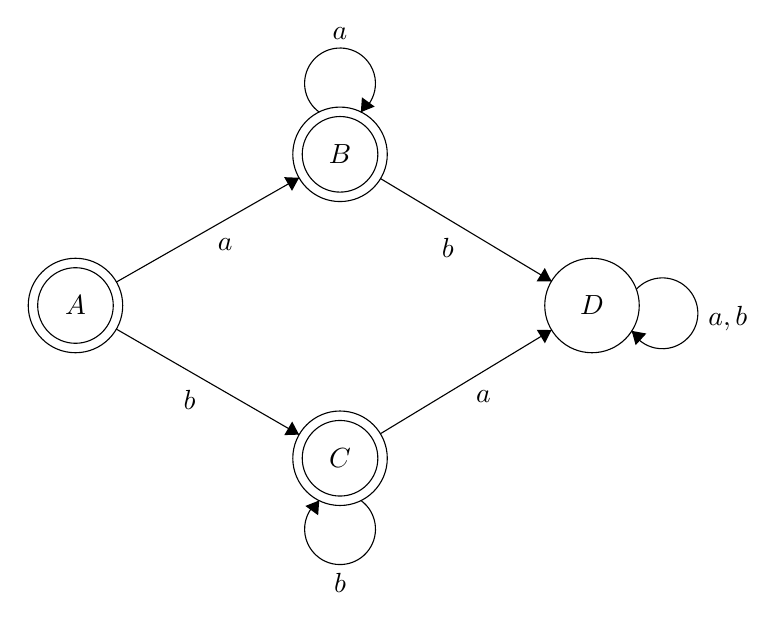
\begin{tikzpicture}[scale=0.2]
\tikzstyle{every node}+=[inner sep=0pt]
\draw [black] (16.7,-26.4) circle (3);
\draw (16.7,-26.4) node {$A$};
\draw [black] (16.7,-26.4) circle (2.4);
\draw [black] (33.5,-16.8) circle (3);
\draw (33.5,-16.8) node {$B$};
\draw [black] (33.5,-16.8) circle (2.4);
\draw [black] (49.5,-26.4) circle (3);
\draw (49.5,-26.4) node {$D$};
\draw [black] (33.5,-36.1) circle (3);
\draw (33.5,-36.1) node {$C$};
\draw [black] (33.5,-36.1) circle (2.4);
\draw [black] (19.3,-24.91) -- (30.9,-18.29);
\fill [black] (30.9,-18.29) -- (29.95,-18.25) -- (30.45,-19.12);
\draw (26.2,-22.1) node [below] {$a$};
\draw [black] (36.07,-18.34) -- (46.93,-24.86);
\fill [black] (46.93,-24.86) -- (46.5,-24.02) -- (45.98,-24.87);
\draw (40.35,-22.1) node [below] {$b$};
\draw [black] (32.177,-14.12) arc (234:-54:2.25);
\draw (33.5,-9.55) node [above] {$a$};
\fill [black] (34.82,-14.12) -- (35.7,-13.77) -- (34.89,-13.18);
\draw [black] (34.823,-38.78) arc (54:-234:2.25);
\draw (33.5,-43.35) node [below] {$b$};
\fill [black] (32.18,-38.78) -- (31.3,-39.13) -- (32.11,-39.72);
\draw [black] (52.309,-25.381) arc (137.65981:-150.34019:2.25);
\draw (56.86,-27.25) node [right] {$a,b$};
\fill [black] (52.02,-28.01) -- (52.27,-28.92) -- (52.95,-28.18);
\draw [black] (19.3,-27.9) -- (30.9,-34.6);
\fill [black] (30.9,-34.6) -- (30.46,-33.77) -- (29.96,-34.63);
\draw (23.95,-31.75) node [below] {$b$};
\draw [black] (36.07,-34.54) -- (46.93,-27.96);
\fill [black] (46.93,-27.96) -- (45.99,-27.94) -- (46.51,-28.8);
\draw (42.6,-31.75) node [below] {$a$};
\end{tikzpicture}
\end{center}


Using the table filling algorithm, we will prove that the fewest number of states required for a machine to accept $L(R)$ is $4$\\

\begin{tabular}{l|llll}
& A & B & C & D \\
\hline
A & -& $\times$& $\times$ &$\times$ \\
B &$\times$ & -&$\times$  &$\times$\\
C & $\times$ & $\times$ & -& $\times$ \\
D &$\times$ &$\times$ & $\times$ &- \\
\end{tabular} \\ \\

After running the table filling algorithm, we can see that all pairs of states are identified and therefore distinguished.\\
This means that there are no equivalent states in this machine, so this machine cannot be minimized further.\\
So a machine that accepts $L(R)$ as it's language cannot have less than four states.\\
Thus, there cannot exist a DFA $M = (Q, \Sigma, \delta, q_0, A)$ such that $|Q| = 3 \ \wedge \ L(M) = L(R)$

\end{proof}
\end{document}